% !TeX program = lualatex
\documentclass[a5paper,11pt,openany]{article}
\usepackage{orcidlink}

\usepackage{blindtext}
%\usepackage[style]{abstract}

\usepackage[top=2cm,bottom=2cm,bindingoffset=0cm]{geometry}

\usepackage[svgnames]{xcolor} % Required to specify font color

%\documentclass[a4paper,12pt,openany]{scrbook}

%\usepackage{glossaries}
%\usepackage[xindy]{glossaries}
%\makeglossaries

%\usepackage{odsfile,lmodern}

%\usepackage{luacode}


\usepackage{multicol}

%\usepackage{churchslavonic}
%\usepackage{polyglossia}
%\setotherlanguages{russian,churchslavonic}

\usepackage{mathtext}
\usepackage{makeidx}
%\usepackage{imakeidx}
\usepackage{longtable}
\usepackage[tc]{titlepic}

\usepackage{fontspec}

\usepackage[protrusion=true,expansion,
tracking=true,letterspace=50]{microtype}


%\usepackage{academicons}
%\usepackage{xcolor}


%\SetTracking[ spacing = {25*,166, } ]{ encoding = *, shape = sc }{ 25 }


%\usepackage{soulutf8}
%\usepackage{letterspace}

%\usepackage[toc]{appendix}
\usepackage[toc,titletoc]{appendix}
\renewcommand\appendixtocname{Приложения}
\renewcommand\appendixpagename{Приложения}

%\usepackage{xunicode}
\usepackage{xltxtra}

\usepackage[normalem]{ulem}
\usepackage{adjustbox}

\usepackage{polyglossia}
\setmainlanguage{russian}
\setdefaultlanguage{russian}
\setotherlanguage{ukrainian}
\setotherlanguage{english}
\setotherlanguage{greek}
\setotherlanguage{latin}
\setotherlanguage{polish}


\setmainfont[BoldFont={DejaVuSerif-Bold.ttf},
ItalicFont={DejaVuSerif-Italic.ttf},
 BoldItalicFont={DejaVuSerif-BoldItalic.ttf}]{DejaVuSerif.ttf}

\setromanfont[BoldFont={DejaVuSerif-Bold.ttf},
ItalicFont={DejaVuSerif-Italic.ttf},
 BoldItalicFont={DejaVuSerif-BoldItalic.ttf}]{DejaVuSerif.ttf}

\setsansfont[BoldFont={DejaVuSans-Bold.ttf},
ItalicFont={DejaVuSans-Oblique.ttf},
 BoldItalicFont={DejaVuSans-Oblique.ttf}]
{DejaVuSans.ttf}

\setmonofont[BoldFont={DejaVuSansMono-Bold.ttf},
ItalicFont={DejaVuSansMono-Oblique.ttf},
 BoldItalicFont={DejaVuSansMono-BoldOblique.ttf}]
{DejaVuSansMono.ttf}



\usepackage{enumitem}
\usepackage{indentfirst} 

\usepackage{verse}

\usepackage{graphicx}

%\usepackage[pdfpagelabels,unicode,plainpages=false]{hyperref}

\hypersetup{pdftitle=Скотий бог Волос. Петр Семилетов.}

\usepackage{bookmark} 
\usepackage{relsize}

\usepackage{tocloft,calc}
\usepackage[nottoc,numbib]{tocbibind}


\frenchspacing
\righthyphenmin=2


\makeatletter
\@addtoreset{chapter}{part}
\makeatother  


%\titlepic{\includegraphics[width=0.50\textwidth]{cover/04.jpg}}

\title{CКОТИЙ БОГ ВОЛОС\\
\textsmaller[2]{редакция 1.0}}
\author{Петр Семилетов\\ORCID:0009-0002-3901-7785 \orcidlink{0009-0002-3901-7785}}
\date{24/11/2024}



\newcommand*{\plogo}{\fbox{$\mathcal{PL}$}} % Generic publisher logo

% –  –  –  –  –  –  –  –  –  –  –  –  –  –  –  –  –  –  –  –  –  –  –  –  –  –  –  –  –  –  –  –  –  –  –  –  –  –  –  –  –  –  –  – 
%	TITLE PAGE
% –  –  –  –  –  –  –  –  –  –  –  –  –  –  –  –  –  –  –  –  –  –  –  –  –  –  –  –  –  –  –  –  –  –  –  –  –  –  –  –  –  –  –  – 

\newcommand*{\titleAT}{\begingroup % Create the command for including the title page in the document
\newlength{\drop} % Command for generating a specific amount of whitespace
\drop=0.1\textheight % Define the command as 10% of the total text height

\rule{\textwidth}{1pt}\par % Thick horizontal line
\vspace{2pt}\vspace{-\baselineskip} % Whitespace between lines
\rule{\textwidth}{0.4pt}\par % Thin horizontal line

\vspace{\drop} % Whitespace between the top lines and title
\centering
\textcolor{Red}{
{\Huge СКОТИЙ БОГ ВОЛОС}\\[0.5\baselineskip] % Title line 1
%{\Large}\mbox{}\\[0.75\baselineskip] % Title line 2
%{\Huge четвертая редакция}} % Title line 3
}

\vspace{0.25\drop} 
\rule{0.3\textwidth}{0.4pt}\par 

\mbox{ }\\
редакция 1.0\\

%\includegraphics[width=0.40\textwidth]{cover/04.jpg}

\vspace{\drop} 

{\Large \textsc{Петр Семилетов\\ORCID: 0009-0002-3901-7785}}\par 


\vfill
%{\large \textcolor{Red}{\plogo}}\\[0.5\baselineskip] % Publisher logo
{\large \textsc{2024}}\par % Publisher

\vspace*{\drop} 

\rule{\textwidth}{0.4pt}\par
\vspace{2pt}\vspace{-\baselineskip} 

\rule{\textwidth}{1pt}\par 

\endgroup}


\begin{document}


\maketitle

\pagestyle{empty}


\newpage

\pagestyle{plain}

%\hrule

%\tableofcontents

%\input{pre/pre.tex}
%\input{plan-right/plan-right.tex}
%\input{plan-right/plan-right-text.tex}

\begin{abstract}
Где в Киеве стояло капище языческого бога Волоса? Какие христианские святые приобрели в представлениях народа свойства Волоса как покровителя домашних животных? Как Волос связан с киевским урочищем Выдубичами и крещением Руси?
\end{abstract}


\section{КИРИЛЛ И МЕФОДИЙ - НЕ ИЗОБРЕТАТЕЛИ!}

С Кириллом и Мефодием, точнее Константином (Кириллом он стал, приняв схиму) и Мефодием, деятельных братьев из Солуни\footnote{Селунь, Солунь – греческий город Салоники.} принято связывать изобретение славянской письменности, алфавита, когда из Моравии поступил запрос на понятную народу Библию, не греческую, не латинскую, но славянскую.

До революции 1917 года, тексты летописей были доступны немногим, да и в советское время переиздавались нечасто. Для работы с ними приходилось ездить в библиотеки Москвы, Киева или Ленинграда, большинство же исследователей довольствовалось разрозненными цитатами, переходящими из книги в книгу, и осовремененными «переводами» летописей, в частности Повести временных лет.

Хрестоматийный перевод Повести временных лет, выполненный Дмитрием Лихачевым, в месте про Кирилла и Мефодия, гласит: 

\begin{quotation}
Был един народ славянский: славяне, которые сидели по Дунаю, покоренные уграми, и моравы, и чехи, и поляки, и поляне, которые теперь зовутся русь. Для них ведь, моравов, первых созданы буквы, названные славянской грамотой; эта же грамота и у русских, и у болгар дунайских.
\end{quotation}

Открываем подлинник по Лаврентьевскому списку, за 6406 год от сотворения мира:

\begin{quotation}
бе един язык Словенеск. Словени же седяху по Дунаеви ихже прияша Оугри и Марава Чеси и Ляхове и Поляне яже ныне зовомая Русь сим бо первое преложены книги Мараве . яже презвася грамота Словеньская. яже грамота есть в Руси и в Болгаре Дунаиских.
\end{quotation}

Где тут написано про создание букв? Откуда Лихачев взял, что для Моравов\footnote{Кстати, Моравы сами себя еще в 19 веке именовали Чехами. Моравами их называли чужестранцы.} первых созданы буквы, названные Словенской (Славянской) грамотой?

Подлинник ясно говорит – книги (а речь идет о священных христианских книгах, Библии) сперва были «преложены» – переведены – народу Мараве. 

Эти-то переводы называли грамотой Словенской, Писанием Словенским. Опять-таки летописец подразумевает Библию, на Словенском. И дополняет, что такое Писание в ходу в Руси и у Болгар Дунайских. 

Примечательно – еще с 19 века исследователи заметили, что в старейших редакциях житий святых Кирилла и Мефодия на старославянском, сказано «книги», а в поздних «книги» постепенно превращаются в «письмена». Несмотря на это, наука считает Кирилла и Мефодия создателями славянской азбуки, одного из двух алфавитов – кириллицы и глаголицы, еще не пришли к мнению, какого именно. 

%Я сейчас не касаюсь общепринятого положения о том, что Кирлл и Мефодий еще и придумали особый язык

Именно «письмена», или даже «грамота», упомянуты в единственных на греческом языке сочинениях, касаемых Константина и Мефодия – вариантах жития святого Климента, где есть «граммата Скловениха». И слово «γράμματα» («граммата») обычно переводят как «буквы», совершенно выпуская из виду, что оно обозначает и Письмо в смысле Писание, священные книги. Так, на греческом, Iερά Γράμματα – Иэра Граммата, Заветные буквы, Завет, Библия!

А была известна, например, Латинская Библия – Библия на латинском языке. Никто не утверждает же, что Латинская Библия – это название азбуки. Точно также и Словенская Грамота, Словенское Писание – это Библия на словенском, общем тогда славянском языке, который в несколько искаженном по мере переписывания виде дошел до нас в летописях.

В большинстве источников – летописях, житиях, письмах – не сказано, что братья создавали азбуку. «Повесть временных лет», говоря о Кирилле и Мефодии, отрывочно и путано пересказывает их жития, но поскольку именно летописное изложение событий известно больше других, разберем сначала его.

Согласно «Повести», правители Славян, живущих по Дунаю – князья Ростислав, Святополк и Коцел – просят византийского царя Михаила снабдить их крестившихся подданных переводами священных книг\footnote{Прежде они просили о том же папу Адриана II, однако не успел он послать своих людей, как дело перехватил Михаил.}, ибо, по Ипатьевскому списку,

\begin{quotation}
не разумеем бо ни Гречьскому языку, ни Латыньскому, оны бо ны инако учать, а друзии инако; темьже не разумеем книжнаго разума, ни силы их; а послете ны учителя, иже могуть ны сказати книжная словеса и разум их
\end{quotation}

Князья хотят малого – переводчиков священных христианских книг, уже проповедуемых среди Словен (Славян) на латыни и греческом, которые народу непонятны. Не сказано, что Словене не разумеют родной грамоты. Они не понимают латыни и греческого.

Напомню, что «Византия» это введенное в науке название Римской империи того времени, когда столицу ее перенесли из Рима в Новый Рим (он же Константинополь, ныне Стамбул). В летописях Константинополь именуется Царьградом. Римская империя того времени дала сильный крен в сторону Греции, посему то, что наука окрестила Византией, в наших летописях и житиях упоминается как Греки\footnote{Также в ходу слово «гречник» вместо «грешник», не потому ли что дохристианские греки-эллины были язычниками, и язычник стало синонимом грешнику?}. «Византийцы» же именовали себя Ромеями. 

Византийский царь Михаил просит друнгария\footnote{Должность военного командира в Византии, значение менялось в зависимости от времени.} Льва из Селуни отрядить в словенские земли сыновей – Мефодия и Константина, по прозвищу Философа\footnote{Михаил, сын Феофила, давно был знаком с Константином. Ведь когда умер отец Михаила и последний вступил на престол с матерью своей Феодорой, при нем были, как выражается житие, «пестуны» – великие боляре – доместик Мануил, Феокист патрикий, да логофет Дромн. Дромн знал родителей Константина и Мефодия, и присоветовал Константина в качестве учителя для царя Михаила. Так Константин приблизился ко двору.}. Лев соглашается,

\begin{quotation}
и послаша я\footnote{«Я» значит «их». В подобных выражениях также, после глагола, «и» – его, «ю» – ее. Например, «и послаша и по грибы» – и послали его по грибы.} в словеньскую землю к ростиславу и святополку и кцьлови. сима же пришедшима начаста съставливати письмена азбуковьная словеньски и переложиста апостол и еуангелие, ради быша словене яко слышиша виличья божия своим языком по сем же приложиста Псалтирь и Октаик и прочая книги.
\end{quotation}

Всего-то сказано, по Ипатьевскому списку, что Константин и Мефодий пришли к Словенам да принялись за работу, о которой их просили.  «Съставляти письмена азбуковная словеньски» значит не составили азбуку, как думают, но указание, что братья создали\footnote{Составление можно понимать буквально, ибо Библия ведь составлена из множества книг Ветхого и Нового Завета. И состав этот в давнее время разнился. Более того, к числу священных книг иногда добавлялись непривычные нам произведения, например о Троянской войне.} Писание (письмена) на словенском алфавите, приложив-переложив – переведя – книги Апостол и Евангелие, а затем Псалтирь, Октаик и прочие книги. А Словене «ради быша» – рады были, что услышали хвалу богу своим языком. 

Дальше в летописи идет текст, в котором ученые находят подтверждение своему мнению о Кирилле и Мефодии – создателях славянской азбуки. Некие люди, проведав о переводе священных книг на славянский, были недовольны, и говорили, что

\begin{quotation}
яко не достоин никоторому же языку имети буков своих разве Евреи и Грек и Латины по Пилатову писанию
\end{quotation}

Это предложение в разных вариантах, где читается то «буков», то «азбуков», толкуется следующим образом – мол, недовольные люди утверждали, будто ни один язык, кроме еврейского, греческого и латинского, не достоин иметь своих букв, алфавитов. Здесь «язык» употреблен в значении «народ». 

Слово же «бук» – что это такое? Буква? Кстати, прежде буквой называли и целое слово. Но буква ли «бук»? Заметим – «буки» тут во множественном числе.

В Тверском списке толкуется: «буков своих, рекше, книг» – слово «буки» отождествляется с «книгами».

Я предположу, как толковать происхождение этого слова. Слово «бук», или «боук», похоже на «бок». «Бок» значит – «сторона». Привычное русское слово «страница» по-украински звучит как «сторінка». А «сторінка» – от той же «стороны». Таким образом «буки» это значит просто «страницы».

В Тверском списке «буки» уравнены с «книгами». Всем знакомо английское слово «book» – книга! Полагаю, такое же было и в давнем славянском, но уже во время составления Тверского списка оно устарело, поэтому переписчик дает пояснение – буков своих, рекше, книг. В старину и слово было такое, «букарь» (боукарь) – книжник.

О каком же именно недовольстве говорит летопись, в переложении на современный язык?

Дело проясняют жития святых. Римская ветвь христианской церкви тогда разрешала в богослужении использовать только три языка – латинский, греческий и еврейский, которыми по приказу Пилата были сделаны надписи на кресте Иисуса. Молиться на языке народа, проповедовать – можно\footnote{В православии это получило название «ереси триязычия», в католичестве – триязычной догмы, от которой позже отказались.}. Совершать богослужение, литургию – нет. А Константин и Мефодий сделали перевод Библии и церковных служб на словенский, ныне старославянский, язык.

Греческое слово «βιβλία» – Библия – в переводе означает «книги». Словенскую Библию получили Словене! И духовенство римской церкви возмутилось!
 
Константин затем «взвратився вспять и иде оучить болгарского языка», что означает  – вернулся назад и пошел учить, в смысле проповедовать христианство, а учить кого? – болгарского языка, то бишь болгарский народ.

Мефодий же остался в Мораве, затем князь Коцел назначил его епископом в Пании (Паннонии). И вот странность – Мефодий

\begin{quotation}
посади два попа борзописца велми, и преложи вся книгы исполнь от Грецька языка в Словенеск шестью месяц, начен от марта месяца до двунадесяту и шесть дний октября месяца
\end{quotation}

Если пользоваться сведениями только Повести временных лет, то кажется, будто речь идет о выполнении двух разных переводов. Сначала одного (когда «переложиста апостол и еуангелие»), а потом другого, с греческого языка. Последний перевод занял у Мефодия и двух попов-борзописцев шесть месяцев.

Пожалуй надо теперь расширить круг источников, чтобы изложить события более ясно. Источники – различные варианты житий, да латинские документы, в основном письма римских пап.

Предварительные сведения. Жития святых, Кирилла и Мефодия, известны только на старославянском языке. Принято считать, что это переводы с греческого. Однако житий солунских братьев на греческом не существует. «Не дошли до нас», – утверждает наука.

Равным образом Константин и Мефодий не существуют в византийских документах, хотя братья начинали деятельность свою именно от «восточной», «греческой» ветви христианской церкви, судя по житиям выполняли важные поручения религиозно-дипломатического свойства, и должны быть хоть как-то отражены. Нет.

На греческом языке братья упомянуты только в связи со святым Климентом, в «Пространном житии Климента» болгарского архиепископа Феофилакта, да «Кратком житии святого Климента» архиепископа Димитрия Хоматиана. Первое датируют 11-12 веком, второе – 13-м.

Таким образом основные сведения о Константине и Мефодии известны только по житиям на старом славянском языке и по письмам на латыни.

Константин, при патриархе Фотии и Льве Математике, получил образование в Царьграде:

\begin{quotation} 
Егда же прииде Царю Градоу, ведаше его оучителем да се оучить, и в три месеце навыке граматикию по пррочая се еть оучения. И наоучи се Омироу\footnote{Омир – Гомер.} и геометрии. и оу Льва и у Фотия диалезнице и всем философинскыим оучением, к сим же и риторики и арифьмитикии, астрономии и моусикии, и вьсем прочиим елиньскым хоудожеством.
\end{quotation} 

На Константина обратили внимание при дворе, а чтобы удержать философа от монашества, его назначили библиотекарем у патриарха, в «светеи Софии». Но вскоре Константин вышел на «Оузькое море» и там тайно скрылся в монастыре. Впрочем его нашли.
 
Спустя некоторое время император Михаил послал Константина с миссией в Козаре, поскольку тамошний правитель попросил у Византии представителя христианской религии для участия в выборах Козарами как бы государственной религии. Ибо иудеи да сарацины уже начали склонять Козар в свою пользу. И козарский царь не знает, что делать. Сарацины вот уже дары присылают.

Константин отправляется в Козаре, взяв с собой и старшего брата своего, монаха Мефодия. Прежде того Мефодий был военачальником, приближенным к византийскому императору Михаилу Триглавому (деду «нынешнего» Михаила), но при сыне его Феофиле оставил «мир» и на Афоне постригся в монахи – вероятно, попав в опалу. Теперь же Мефодий «шед слоужи яко раб меньшю братоу, повиноуя ся емоу».

Братья добираются до Херсона, как тогда называли известный нам Херсонес, а купно и его окрестности, достаточно большую часть Крыма. Чтобы не путать вас в названиях, ведь современный континентальный Херсон просто носит то же имя, что давний крымский, Таврический, буду вместо последнего Херсона писать Корсунь, как его часто и называли Славяне.

По ранним житиям можно понять, что Корсунь подчинялась Козарам. По более поздним, скажем, 18 века – Корсунь просто смежна козарским владениям. С течением времени так оно и было, город был то под одним государствам, то под другим. 

В истории принято считать, что Корсунь в 9-м веке вошла в состав Священной Римской Империи. Корсунь с некоторых пор играла важную роль в христианской церкви, сюда часто ссылались насильно, либо бежали добровольно изгои, попавшие в очередную бурю византийских религиозных дел. Допустим, шли гонения на иконопочитание – гонимые обретали пристанище в Корсуни.

Там-то, Константин обучается «жидовьсцеи беседе и книгам». «Некий самаренин» снабжает Константина «книгами самаренскими», философ удивляет того своим знанием языка, читая их без запинки.

Далее происходит странное – про Константина, в житии его сказано\cite{teodorov01}:

\begin{quotation}
Обреть же тоу еваггелие и псалтырь росьскы писмены писано, и человека обреть глаголюща тою беседою: и беседовав с ним и силоу речи приемь, своеи беседи прикладая, разоучи писмена гласьная и сьгласная, и к богоу моливою дрьже в скоре начеть чисти и ськазати.
\end{quotation}

Каким-то образом Константин «обрел» – приобрел, купил ли, получил в подарок – Евангелие и Псалтырь (псалмы из Ветхого завета), писанные росьскими письменами, да нашел знающего ту речь (беседу) человека. Общаясь с ним, Константин вскоре выучился читать и говорить по-росьски.

Это относится ко времени предшествующему тому, когда Константину и Мефодию поручили переводить Библию на словенский. Казалось бы, можно воскликнуть – так вот в чем разгадка последующего быстрого перевода!

Но тут загвоздка. Понятие «народа Руси» в то время очень размыто. Каких Русов имеет в виду сочинитель жития? 

С определенного времени Русами стали называть славянские народы, подчиненные тем Русам, что пришли вместе с Рюриком и его родственниками сначала в нынешнюю Новгородщину, а затем ниже до самого Киева. Откуда были те, первоначальные Русы - с Балтики ли, или еще дальше, дело сложное и сейчас стороннее. А давние арабские путешественники говорят о Русах, что живут в крепости на острове в море (иногда уточняется – Меотийском, то бишь современном Азовском), и что остров тот три дня длиной, царь же Русов называется «хакан-рус», что сближает его с козарским «каганом». 

Слово «хакан» всплывает также во франкской хронике Annales Bertiniani, где говорится о посольстве от византийского василевса Феофила к Людовику Благочестивому (что датируется 839 годом нашей эры). В составе посольства были представителя народа «Рос», и правитель их, согласно хронике, назывался «хакан». 

Русы, про которых пишут арабы, постоянно крутятся у низовий Волги, и вообще по морям, широтой близких к Средиземноморскому. При этом арабы различают Русов и Славян.

По житию Мефодия, цесарь Михаил, позже отправляя братьев в Моравию, к Славянам, говорит: «вы бо еста селоунянина, да селоуняне вьси чисто словеньскы беседоують» – то есть вы селуняне, а все селуняне говорят почти как Славяне.

Исходя только из жития Константина, нельзя однозначно понять, каковы были «росьскы писмены», на коем написаны «обретенные» Евангелие и Псалтырь, но по рассуждению сочинителя жития, Константину понадобился носитель языка, дабы в них разобраться.

%Затем, не менее загадочным образом Константин «обретает» святыню – мощи святого Климента, папы римского, умерщвленного в корсуньской ссылке\footnote{«Игемон Авфидиан» по приказу кесаря Траяна утопил Климента, привязав к его шее якорь. С морской гробницей Климента связано множество чудесных преданий. По совокупности их я предполагаю, что гробница находилась на острове, время от времени затопляемом.}. Житие описывает это так\footnote{Существует и отдельное предание про обретение мощей Климента. Позже мощи эти князь Владимир Красно Солнышко, крестившись в Корсуни, забрал с собой.}:

Затем, не менее загадочным образом Константин «обретает» святыню – мощи святого Климента, папы римского, умерщвленного в корсуньской ссылке\footnote{«Игемон Авфидиан» по приказу кесаря Траяна утопил Климента, привязав к его шее якорь. С морской гробницей Климента связано множество чудесных преданий.}. Житие описывает это так\footnote{Существует и отдельное предание про обретение мощей Климента. Позже мощи эти князь Владимир Красно Солнышко, крестившись в Корсуни, забрал с собой.}:

\begin{quotation}
Слышав же яко светыи Климент иже в мори лежить, помоливь се рече: вероую в бога и светем Клименте надею се, яко обрести его имамь и изнести из моря.
\end{quotation}

То бишь, Константин слышал, что прах святого Климента в море лежит, и философ с божьей помощью надеется найти его и достать из моря. Не в одиночку:

\begin{quotation}
Оубеждь же арьхиепискоупа\footnote{Житие Кирилла и Мефодия от Дмитрия Ростовского называет его «епископом Херсонским» Георгием Блаженным.}, и с клиром вьсемь и говеины моужи вьседьше в корабль идоше на место, и оутиьшоу се море вельми и дошьдыше начеше копати поющи. Абие же бысть хризма многа яко и кадиль многь.

О по сем явише се светые мощи, еже вьзьмьше сь великою чьстию и сь славою вьсехь граждан вьнесоше вь град также пишеть в обретении его.
\end{quotation}

После деятельности в Козарах, где братьям удалось крестить тамошнего кагана\footnote{В качестве миссионеров в Козарах солунские братья оставили священников из Корсуни.}, бояр его, а также часть простого народа, Мефодий получает первое «повышение по службе» – назначается от греческой церкви игумном в монастырь Полихрон.

Проходит время. Из Моравии от князей Ростислава и Святополка поступает известный запрос, насчет прислать «учителей» и толковать христианское Писание на народном, славянском языке. Согласно некоторым житиям, князья хотят видеть Константина и Мефодия именно потому, что знают об их успехе в Козарах.

Но тут задача сложнее – нужна Славянская Библия, на славянском, словенском языке. Царь Михаил и дядя его Варда поручают Константину этому способствовать – найди, мол, способ перевести. Бог даст! Не смея ослушаться «ни бога, ни цесаря», Константин помолился, и 

\begin{quotation}
в скоре же емоу бог яви послоушание молитв своих раб: и абие сьложи писмена. и начет беседоу писати еваггельскоу: исперва бе слово, и слово бе оу бога, и бог бе слово, и прочее.
\end{quotation}

По другому варианту жития,

\begin{quotation}
да тоу яви бог философу словеньскы книгы
\end{quotation}

Обрадовался Михаил столь скорому и чудесному явлению перевода Священного Писания.

Константин и Мефодий отправились в Моравию, где Константин взял на обучение людей, выделенных Ростилавом. Вскоре Философ перевел «весь церковный чин» и обучил ему учеников:

\begin{quotation}
В скоре же весь церьковьный чин преложь наоучи и, оутрьници, часовомь и вечерьни, павечерници и таинеи слоужьбе.
\end{quotation}

Яко же рекохом преже, это вызвало недовольство внутри римской церкви, однако разбор интриг, которые на этом не закончились, оставляю вне этой книги\footnote{Недовольство проявляли латинские и франкские архиереи, иереи и ученики их. Константин вступал с ними в споры. Эти же архиереи, по житию, были в некотором роде язычниками. Они утверждали, что под землей живут «человеци велеглави» (люди с большими головами), а что если кто убьет змею, ему отпустятся девять грехов, ежели же человека убьет, то довольно три месяца пить из деревянной чаши, не касаясь стеклянной – и грех тоже сойдет, как с гуся вода. Архиереи-противники Константина не запрещали язычникам приносить их жертвы, и позволяли неограниченно соединяться в браке. А Константин разводам противился.}. Думаю, что недовольство было вызвано не столь догматом «триязычия», сколь возрастающей популярности варианта учения, предлагаемого Константином и Мефодием на местном языке. Братья пришли со Словенским Писанием в руках да с молитвой «Отче наш» вместо «Pater noster» на устах. Конечно, народ потянулся к ним.

Обстановка вокруг братьев накалилась. Но князь Коцел попросил у римского папы послать к себе «блаженного учителя нашего», подразумевая Мефодия.

Солунские братья отправились в Рим с мощами святого Климента. Это приблизительно совпало по времени с назначением римским папой Андрианом II Мефодия на должность епископа Моравии и Паннонии. Андриан II

\begin{quotation}
книгы словенские освети, и положи и вь церькви светые Марие, яже наричеть се Фатань, и пеше над ними светоую литоурьгию. По сем повеле папа двема епископома, Фоурьмосоу и Гондрихоу, светити словенские оученикы: и якоже светише се, абие пеше литоургию в церкви светаго апостола Петра словеньскыим языкомь.
\end{quotation}

Римский папа осветил «книгы словенские» –  Библию Словенскую – и положил их в церкви святой Марии, и пел над ними святую литургию. Затем он повелел епископам Фурьмусу и Гондриху освятить словенских учеников (обученных братьями), и после этого те пели литургию на словенском языке в церкви святого Петра.

Словом, папа дал добро! Но впрочем предписал, чтобы в Моравии на литургии Послания и Евангелие зачитывались сначала по латыни, а потом уже можно на славянском. Следующий римский папа, Иоанн VIII, письмом своим запретил Мефодию богослужения на славянском, однако архиепископ не послушался. Запреты и разрешения следует толковать лишь на фоне тогдашней религиозной и политической обстановки, когда одни ветви церкви были в содружестве с одними правителями, а другие – с другими.

Став архиепископом Моравии и Паннонии, Мефодий завершает перевод на словенский язык тех книг Писания, которые еще не переведены. Именно из этой части жития Мефодия взято в Повесть временных лет про попов-борзописцев. За шесть месяцев, с греческого на словенский, переводят все оставшиеся книги, кроме Маккавеев: 

\begin{quotation}
Потом же отверг вься молитвы и печаль свою на бога възложи, преже же от оучеников своих посажь два попы скорописьца зело, преложи в борзе вься книгы – вься исполне, разве Макавеи – от грьчьска языка в словенеск шестью месяц, начьнь от марда месяца до дъвоюдесятоу и шестию день октября месяца. Оконьчавь же достоиною хвалою и славою богоу воздасть, дающемоу таковоу благодать и поспех; и святое возношение таиное с клиросом своим вознес сотвори память святаго Димитриа.

Псалтирь бо бе тъкъмо и евангелие с апостолом и избраныими слоужьбами церковьныими с философом преложив первее. Тогда же и номоканон, рекьше законоу правило, и отеческыя книгы преложи.
\end{quotation}

В последнем абзаце важно – Псалтырь и Евангелие, да некоторые избранные службы, были переведены раньше, еще вместе с Константином Философом. 

А ведь именно Константин в Корсуни «обреть же тоу еваггелие и псалтырь росьскы писмены писано». Если сопоставить не мудрствуя лукаво, то выходит, что царю Михаилу был представлен тот самый готовый перевод, «обретенный» в Корсуни. А точнее, если принимать за истину события жития, то переложенный с «росьскы писмены» на словенский, славянский. Поскольку, судя по всему, языки несколько отличались и Константину пришлось учиться у носителя. Но выходит, в любом случае, что так было проще, нежели переводить с греческого, латыни или древнееврейского.

Проложное\footnote{Пролог – древнерусская книга-месяцеслов. Жития святых в нем упорядочены по дням поминовения.} Житие Константина и Мефодия (стык 13-14 веков), уточняет временную привязку перевода, выполненного Мефодием:

\begin{quotation}
Седеше в земли Моравьстеи, преложи вься книгь ветьхаго и новааго закона от гречьскаго вь словенськый, в 3 индикт в 6 тисоущное триста 4 го ста третие лето при Святополца князы; цесарь беше грьчьскы Василие, а бльгаромь от бога князь Борысь, краль немечьскый Людемь.
\end{quotation}

В 879 году недовольство римского руководства деятельностью Мефодия достигло предела. Папа Иоанн VIII вызвал Мефодия на суд в Рим, обвиняя в ереси. Мефодий подчинился, но суд оправдал Мефодия, а папа признал возможность славянского богослужения и непротиворечие его обычаям римской церкви. Судили довольно странно, келейно. Вопреки всему, по поводу Мефодия не созывался синод, поскольку сохранились акты синода за 879 и 880 годы. Всё решилось самим папой и «братьями»-епископами.

Тот же папа в послании князю Святополку, в подтверждение архиепископства Мефодия (Iohannes VIII papa ad Svyatopolcum comitem. Confirmat Methodium ijn archhieposcopatu Moravie, Vichinum facit episcopum Nitriensen at Linguam sclavicam in missis celebrandis adhi\-bendam permittit) сообщает:

\begin{quotation}
\begin{otherlanguage}{latin}
Litteras denique sclavonicas a Constantino quondam philosopho repertas, quibus deo laudes debite resonent, jure laudamus, et in eadem lingua Christi domini nostru preconia at opera ut enarren\-tru jubemus.
\end{otherlanguage}
\end{quotation}

Если у кого доходят руки до этого документа, обычно толкуют исходя из представлений, что Константин изобрел некую письменность. Исследователь сего вопроса Василий Алексеевич Бильбасов в книге «Кирилл и Мефодий по документальным источникам»\cite{bilbasov} дает следующий перевод:

\begin{quotation}
Наконец, славянские письмена, некогда изобретенные Константином Философом, для того чтоб ими возглашались должныя хвалы Богу, мы справедливо похваляем, и мы приказываем, чтобы на этом языке были излагаемы проповеди и деяния Господа нашего Христа.
\end{quotation}

Но слово «litteras», толкуемое Бильбасовым как «письмена», и «repertas», толкуемое как «изобретенные», переводятся иначе.

«Repertas» – найденные, обнаруженные, обретённые.

«Litteras» – Писания. Вот пример употребления этого слова из Латинской Библии, Евангелие от Иоанна, 7,15:

\begin{quotation}
\begin{otherlanguage}{latin}
et mirabantur Iudaei dicentes quomodo hic litteras scit cum non didiceri  
\end{otherlanguage}
\end{quotation}

Что означает:

\begin{quotation}
И дивились Иудеи, говоря: как Он знает Писания, не учившись? 
\end{quotation}

А вот из 2-го послания апостола Павла Тимофею 3,15:

\begin{quotation}
\begin{otherlanguage}{latin}
et quia ab infantia sacras litteras nosti quae te possint instruere ad salutem per fidem quae est in Christo Iesu.
\end{otherlanguage}
\end{quotation}

Перевод:

\begin{quotation}
Притом же ты из детства знаешь священные писания, которые могут умудрить тебя во спасение верою во Христа Иисуса. 
\end{quotation}

«Litteras» вообще принимало много значений – это и обычные письма, и расписки, и книги, и Писание. В случае Константина речь ведь идет о Славянской Библии. Римский папа говорит про Славянское Писание, Славянскую Библию, которую «нашел» Константин. Как нашел, дело десятое – в Корсуни ли, в Козарах, либо как-то еще.

В одном из вариантов «Похвалы Кирилу и Мефодию» (похвалами называют краткие жития святых) говорится:

\begin{quotation}
Закон же божии соугоубо преложьша в новыи язык предаста, письмена створиша емоу.
\end{quotation}

Новый язык здесь – новый народ. Для еще одного народа, переложили закон Божий, Писание (не алфавит!) сотворили ему, народу (языку) этому. 

Как же случилось, что Кирилл и Мефодий, из учителей словенского языка – учителей в смысле духовных, христианских учителей словенского народа (языка), уже к 18 веку стали, в церковной литературе, а следом за ней в науке – изобретателями славянской азбуки?

С некоторых пор по славянским рукописным сборникам пошло гулять сочинение «о письменех черноризца храбра».

Старейшим списком его считается сборник Иоанна-Александра, он же Лаврентьевский (не путать с Лаврентьевским списком русской летописи), в котором проставлена дата «в год от сотворения мира 6856, индикта 1», что наука переводит в 1347 год нашей эры. Сборник был написан для «царя болгар и греков Иоанна Александра», и потом кочевал по библиотекам, в 17 веке попал из Афона в библиотеку патриарха Никона, затем на Печатный Двор, а ныне находится в отделе рукописей Российской Национальной Библиотеки.

Короткое сказание «о письменех» известно в многочисленных списках, причем «Храбр» обычно считается именем, хотя таких имен не было, и монахи (черноризцы) подобных имен не носили. Однако «храбра» это, скорее, слово «храбрый», склоненное в винительном падеже согласно старому славянскому языку. Сказание кого? Черноризца храбра, монаха храброго. Но поскольку мне нужно его как-то величать, буду пользоваться именем Храбр.

Считается, что жил он в 9-10 веках, и был едва не современником Кирилла и Мефодия. Язык «сказания» тяжеловесен, некоторые слова поддаются разве что толкованию, однако не прямому переводу.

В самом начале Храбр пишет:

\begin{quotation}
прежде оубо словене неймеху книг. иж чрьтами й резами чьтеху й гатааху погани суще. кръстившежеся, римсками й гръчьскым писмены, нуждаахуся словенскы речь безь оустроения.
\end{quotation}

Разберем по кусочкам.

«Прежде оубо словене неймеху книг». Научный перевод – прежде Словене не имели книг, письменности в привычном понимании слова. Мой перевод – прежде Словене не имели Библии. Ведь «Библия» буквально и переводится как «Книги». 

«Иж чрьтами й резами чьтеху й гатааху погани суще». Научный перевод – будучи погаными (язычниками), Словене читали и гадали чертами и резами. Мое толкование – я не понимаю, что такое «черты и резы» и не могу об этом рассуждать. Больше нигде в источниках не сказано о чертах и резах. Эти черты (черти) и резы имеют отношение к гаданию, если «гатааху» значит «гадали». Нечто из области верований, веры, как и Библия.

Далее Храбр пишет: «кръстившежеся, римсками й гръчьскым писмены, нуждаахуся словенскы речь безь оустроения».

Ученые понимают это так – крестившись, Словене пытались без всяких правил записывать свою речь римскими и греческими буквами.

Допустим, но почему такая острая необходимость в письменности возникла у Славян сразу после крещения? До того они, наверное, скакали с ветку на ветку, оглашая леса дикими криками и довольствуясь гаданием на чертах и резах? А после принятия христианства ощутили потребность писать на родном языке.

По Храбру, до Кирилла и Мефодия, крещеные Словене достаточно долго – «многа лета» – пользовались чужими алфавитами, что было довольно неудобно для выражения слов словенского языка. И потом Бог не оставил «род человеч» (подразумеваются наверное Словене) без «разума» (христианского учения) и послал им святого Константина Философа, нарицаемого Кирила, мужа праведного и истинного, и тот придумал Словенам буквы, взяв за образец греческие и дополнив алфавит под нужды славянского произношения.

Далее Храбр рассуждает о развитии греческой азбуки, как поначалу Эллины переняли ее у Финикийцев, а разные древние ученые мужи постепенно добавляли новые буквы. Но Греки были язычниками, посему создание греческого алфавита длилось «многи лета», а Кирилл – муж Божий, потому изобрел словенскую азбуку в малых летех, причем в одиночку! Несколько далее в своем сказании Храбр впрочем мельком упоминает и Мефодия.

Итак, с одной стороны, у нас есть жития Кирилла и Мефодия, где они не изобретают буквы, но выступают в роли переводчиков, причем Константин-Кирилл, помолившись, вскоре являет Михаилу переведенными на словенский священные книги в том же составе, каковой он «обрел» в Крыму, в Корсуни.

Подобное отношение, к Кириллу и Мефодию как к переводчикам и учителям христианской веры среди Словен (Славян), пронизывает и другие христианские тексты, помимо житий. Например, в поминальных службах, Кирилла величают «учителем словенскому языку», то бишь учителем, просветителем словенского народа. Глас из рукописи С. Палаузова:

\begin{quotation}
Кыриле, славне оучителю! Доброте научи моравлени своими бога благодарити, прелагая на словеньскы языкь от грьчьскаго закон господень, и правде его.
\end{quotation}

На другую чашу весов положим коротенькое сочинение «О письменех» черноризца Храбра, где утверждается без каких-либо доказательств изобретение Константином славянской азбуки на основе греческой, а скорость перевода приписывается тому, что Константин был христианином.

Современные ученые принимают на веру версию монаха Храбра.

Но мало им утверждений, что солунские братья изобрели для диких Славян азбуку. Много лет уже внедряется мнение, что и давний славянский язык, известный нам по дошедшим летописям, житиям и прочим памятникам литературы – в быту не ходил, но использовался сугубо книжно. То есть мало лишить Славян письменности, надо еще и языка исконного лишить! Дескать, его тоже изобрели Кирилл и Мефодий.

%Поминальная по Кирилу и Мефодию, по списку 17 века

%Святый Кирил философ, родом сеи Блъгарин от Солоуна града, грамота новая створи и преложи грьечскыи язык на роусскыа книгы с братом присным своим Мефодием, иже и тъ бысть первыи архиепископ моравский и чешьский, в царьство Михаила, царя гречьскаго и в дни архиепископа Коньстантина града блаженнаго патриарха Фотия, в лета князя блъгарскаго Бориса и Растица бооустнаго князя моравскаго и Костела князя Блатского и Лесскаго и Зубра когана козарскаго, и Карлоуса краля немечьскага, и Доуная господаря угорьскаго, царствуяшему же в Новьграде князю роуському Роурикоу, до 100 20 2 лет

Почему-то никто не проделывает тот же финт ушами с «древнескандинавским», или, правильнее, старым северным (Old Norse) языком. Наукой признается, что на нем говорили «скандинавы» эдак с 8 по 14 века. «Северный германский язык!» – весомо определяет наука. На нем известны некоторые саги, сборники «Эдда» и «Старшая Эдда» и различные рунические надписи. Но ученые не считают, что это был особый такой язык, годный только чтобы сочинять на нем саги. Признают – да, использовался в обиходе.

А с расшифровкой рун иногда получается так. В Эрмитаже хранится арабский динар, датируемый 701/702 годом нашей эры. На нем, помимо арабской вязи, невесть когда нацарапано на старославянском:

\begin{center}
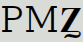
\includegraphics[width=0.20\linewidth]{chast-colebanie-osnov/letyaz/pmz.png}
\end{center} 

Последняя буква – «земля», «з». Ученые берут и толкуют – это не буквы, а руны. «M» – две отдельные руны, а «земля» тоже руна, но без вертикальной палочки. И надпись надо читать: «kut». Засучив рукава, толкователи рун берутся за дело. Одни говорят, что «kut» – окончание имени некоего скандинава! В высшей степени научно. Другие бают – а вот давайте добавим еще букву «r», да поменяем звуки, получится gótr или gautr, что можно было бы перевести как «мужчина» или «воин». Третьи утверждают, что тогда «Gautr» это другое имя бога Одина. Четвертые не согласны, и видят в надписи другие руны – слово «góts», но это если вторая руна длинное – «ó», а последняя – «s».

Итак, ясно вычерченную на монете славянскую надпись ученая братия считает «норманскими» рунами, толком не понимая, какие же именно руны написаны, и предлагает уйму вариантов прочтения.

Вместо того, чтобы задуматься о прочтении письмен старославянских...

Ведь как читали? Разложим вопрос на две части. Способ и произношение.

Способ. 

Как читает грамотный современный человек? Он читает не по буквам, а по словам, зная как они выглядят. Слова для него – картинки. Лишь новое слово постигается вначале побуквенно, что нужно, дабы знать как произносить слово, а потом оно становится цельным изображением. Чтобы различать слова, человек пользуется, упрощенно говоря, пробелами между ними. Это позволяет быстро понять, где начало слова, где конец, а всё что между этим – изображение слова.

В рукописях на старославянском, будь то летописи или религиозные сочинения, слова никак не разделяются, буквы идут сплошными рядами. Это относится и к греческим рукописям, а хоть бы и Нового Завета.

В лучшем случае старославянский писец ставил точки (посередине высоты строки), разделяя логически части предложения, дабы облегчить чтение. При таком положении дел вы не можете быстро найти нужный вам отрывок, не можете постигать написанное пословно, просто глядя на абзац или предложение. Вам нужно читать побуквенно и, дабы не сбиться, водить пальцем  по строкам, будто палец – это курсор. Итак, чтение было не пословное, а побуквенное, и только прочитанная порция букв могла быть сложена в слово, а затем чтец начинал читать следующие буквы, покуда не натыкался на конец слова, если конечно знал его. В случае согласной в завершении слова ставился твердый знак, что указывало на конец слова.

Произношение. Никто не ведает, как говорили на латыни во время, когда ею пользовались в обиходе. Никто не в курсе, как говорили на старославянском. Как вслух читались слова, которые написаны в летописях. Современное духовенство может читать на «церковнославянском», но это осовремененный выговор, приближенный к русскому языку последних нескольких веков.

Как же восстановить произношение времен, например, Нестора Летописца?

Сохранились переводы на старославянский с того же греческого, и перебрасывая мостки между греческим произношением (хотя никто не знает, как тогда произносили написанные слова Греки), можем примерно догадаться о разных вещах.

Буква «Є» – называемая в церковнославянском «есть». В старославянских текстах не встречается привычная нам «Е», но есть такая «Є», как в украинском, где этот знак обозначает как раз русское «е» – «йэ».

Однако, в старославянском, и дореволюционном правописании русского языка, была буква Ѣ (ять).

Очевидно, что держать две буквы для использования одного и того же звука не было нужды, следовательно буквы «Є» и «Ѣ» звучали по-разному. Кстати, до революции использование слов с «Ѣ» просто держали в памяти, толковых правил этому так и не вывели. 

Самоназвание жителей Греции  – Эллины. В летописях оно пишется как «Єллини». Думаю, прежнее произношение буквы «Є» соответствует современному «Э». Не зря она даже пишется как повернутая в другую сторону «Є». В старославянских переводах имен тех же ромейских императоров, пишется «Є», хотя звучали они с современным звуком «Э». Вывод напрашивается сам собой.

«И» (церковнославянская «иже») – и парная ей «І», она же «Ї» (называется «и»). Опять же, было отличие в произношении, как в случае с «Є» и «Ѣ». Вероятно, «И» была более «толстой», ближе к «ы». На ум приходят всё те же летописные «Єллини».

«Г» – я не знаю, отколь повелась твердая «г» почти как «к». Но вот даже во времена Петра I писали «г», а говорили «х». Это проявляется в письменных ошибках Петра I, который писал как говорил – ВыборХ, ПетербурХ. Это объясняет написание имени Юрия Долгорукого в некоторых списках в виде Гюрги, что звучит непривычно жестко на современное произношение, но если читать смягченно, выходит Хюрхи, Юрий.

Лишнее подтверждение былой мягкости «г» – использование ее в передаче иностранных имен и названий, которые в подлиннике звучат с «х» – Гамбург (Humburg), Герберт (Herbert), Гарри (Harry) и так далее. Такое написание могло обоснованно возникнуть лишь во время, когда «г» звучала столько мягко, как соответствующая ей латинская «h». Вспомним, как в старину вместо «история» (history) писали «гиштория», или не испанский, но «гишпанский».

«Оу» – еще одна любопытная штука, сочетание букв, позже перешедшее в обычное «у». Например, «Златооустецъ», «моужъ». Вместе с тем, встречается и одиночное «у» – «служебнии». Поскольку письменный язык отражал устный, значит, некоторые слова так и произносились, и вместо короткого «муж» растягивали «моуж». Сие возможно при довольно неторопливой речи, надо успеть произнести. Потом, с течением лет, веков, речь наверное ускорилась, и «лишнее», трудное произношение отпало в пользу короткого. И коротко превратилось в кратко. Выпадали даже целые слова – «еси» – а у англичан оно сохранилось как «is». Сравните Сие еси и this is. 

Медленная устная речь хорошо согласуется с медленным же чтением сплошных рядов букв. А что, если и мысли в то время протекали медленно? 

%Выдумка заменяет ученым обоснование и в решении других вопросов.



\newpage


\newpage

%\backmatter

%\appendix
%\addappheadtotoc


%\input{appendix/dict.tex}

\begin{thebibliography}{999}
\bibitem{zeleninrusalki}
\emph{Избранные труды. Очерки русской мифологии: Умершие неестественною смертью и русалки}. Зеленин Д. К. Индрик, Москва, 1995.

\bibitem{kak}
\emph{Как Владимир идолов низвергал}. Петр Семилетов, DOI 10.5281/zenodo.14212537

\bibitem{volos}
\emph{Скотий бог Волос}. Петр Семилетов, DOI 10.5281/zenodo.14563494
\end{thebibliography}


\end{document} 